\documentclass[a4paper]{article}
\usepackage{titlesec}
\setcounter{secnumdepth}{4}

\titleformat{\paragraph}
{\normalfont\normalsize\bfseries}{\theparagraph}{1em}{}
\titlespacing*{\paragraph}
{0pt}{3.25ex plus 1ex minus .2ex}{1.5ex plus .2ex}




\usepackage{graphicx}
\usepackage[portuguese]{babel}
\usepackage[utf8]{inputenc}
%opening
	\title{Análise do Sistema \\ Letrinhas \\ APP \& Sistema de Informação }
\author{Projecto de Sistemas de Informação}



\begin{document}

	\maketitle %titulo
  
	\newpage
	\tableofcontents %indice
	\newpage %pagina nova

	 \section{Introdução}%resumo - introdução
		\subsection{Visão Geral do Sistema}
		 
		A questão apresentada ao grupo de trabalho consiste na criação de um sistema que permita a avaliação de alunos do ensino básico, em diversas áreas, nomeadamente fluência na leitura, quer ao nível de palavras, quer de textos completos, entre outros tipo de testes como por exemplo interpretação de sons e/ou imagens, sempre através do recurso a um tablet.\\ 

		O sistema será composto por uma aplicação para dispositivos móveis e o respetivo sistema de informação.

		\subsubsection{Aplicação para tablet}
		A aplicação deverá permitir dois tipos de acessos, o do Professor, para fazer a correção dos testes na própria aplicação e o do aluno que através do interface do tablet deverá realizar os testes propostos pelo professor.
		
		\subsubsection{Sistema de Informação}
		O sistema de informação dá suporte à aplicação, recorrendo a uma base de dados e formulários web.

		\subsection{Objetivos}
		
		O Letrinhas tem como principal objetivo permitir a avaliação dos alunos de uma forma simplificada e com diferentes tipos de registos dessa mesma avaliação.\\
		O aluno através do dispositivo móvel terá acesso aos diferentes tipos de testes que serão submetidos previamente pelo professor e avaliados ou no momento ou posteriormente por este. \\
		O sistema de informação estará acessível ao professor e permitirá não só a introdução dos testes, como a revisão de testes efetuados pelos alunos.  


		
		\subsection{Cliente}
		O cliente é o Agrupamento de Escolas Artur Gonçalves, que através  dos docentes da Cadeira de Projetos de Sistemas de Informação, professor António Manso e professor Pedro Dias fizeram a articulação entre as duas partes.
		
		\newpage
		
		\subsection{Fontes e Material de Referência}
		Para melhor compreensão do conceito, utilizamos como material de referência os seguintes.
		
		\subsubsection{Aplicações para gravação de voz}
		\begin{itemize}
			\item eRecorder (Aplicação para android);
			\item Smart Voice Recorder (Aplicação para Android);
			\item Voice Recorder Pro. (Aplicação para Android);
		\end{itemize}
		
		\subsubsection{Aplicações de tradução(Voz para texto)}
		\begin{itemize}
			\item	ListNote Fala-para-texto Notas (Aplicação para Android);
			\item 	Speach to text (Aplicação para Android);
			\item 	Text to speach - Voice to text (Aplicação para Android);
		\end{itemize}
		
		\subsubsection{Software open source}
		\begin{itemize}
			\item	Mi sound recorder (Aplicação para Android);
			\item	Auphonic Software (Aplicação para Android \& Iphone);
			\item	Android Voice Recognition Tutorial;
			\item 	Rehearsal Assistant (Aplicação para Android);
		\end{itemize}
		
		\subsection{Glossário}
			\begin{tabular}{|l|p{10cm}|}
				\hline Android & Sistema operativo para dispositivos móveis. \\ 
				\hline Open Source & Software Informático que respeita as quatro liberdades definidas pela Free Software Foundation. \\  	
				\hline 
			\end{tabular} 
		
		\newpage %pagina nova
		\section{Modelo de Casos de Utilização}
			\subsection{Atores}
		
			\subsubsection{Aplicação}
				\begin{tabular}{|c|p{10cm}|}
					\hline Ator & Descrição \\ 
					\hline Aluno & Ator do sistema que interage diretamente com a aplicação realizando os testes propostos. \\ 
					\hline Professor & Quem distribui e supervisiona o teste realizado pelo aluno. \\ 
					\hline 
				\end{tabular} 
		
			\subsubsection{Sistema de Informação}	
				\begin{tabular}{|c|p{10cm}|}
					\hline Ator & Descrição \\ 
					\hline Administrador & Ator responsável por criar contas de professor, adicionar escolas e alunos ao sistema. \\ 
					\hline Professor & Ator responsável por manipular o conteúdo da base de dados, criar, corrigir e consultar testes de avaliação. \\ 
					\hline 
				\end{tabular} 				
	
	
			
			
			\subsection{Visão geral}
		O sistema irá implementar as funções acima descritas e outras que são efectuadas automaticamente pelo sistema e como tal não são visíveis nos casos de utilização.\\
		
		Aos recolhidos em levantamento de requisitos foram adicionados certos casos de utilização considerados pertinentes.\\
		
		Abaixo temos os diagramas de casos de utilização para uma melhor  visão e compreensão do sistema.

			
			\newpage
			
			\subsection{Diagramas de Casos de Utilização}
			\subsubsection{Casos de utilização da aplicação}
			
			\paragraph{Diagrama de CaU do ator professor e aluno}
			
			\begin{figure}[h]
				\centering
				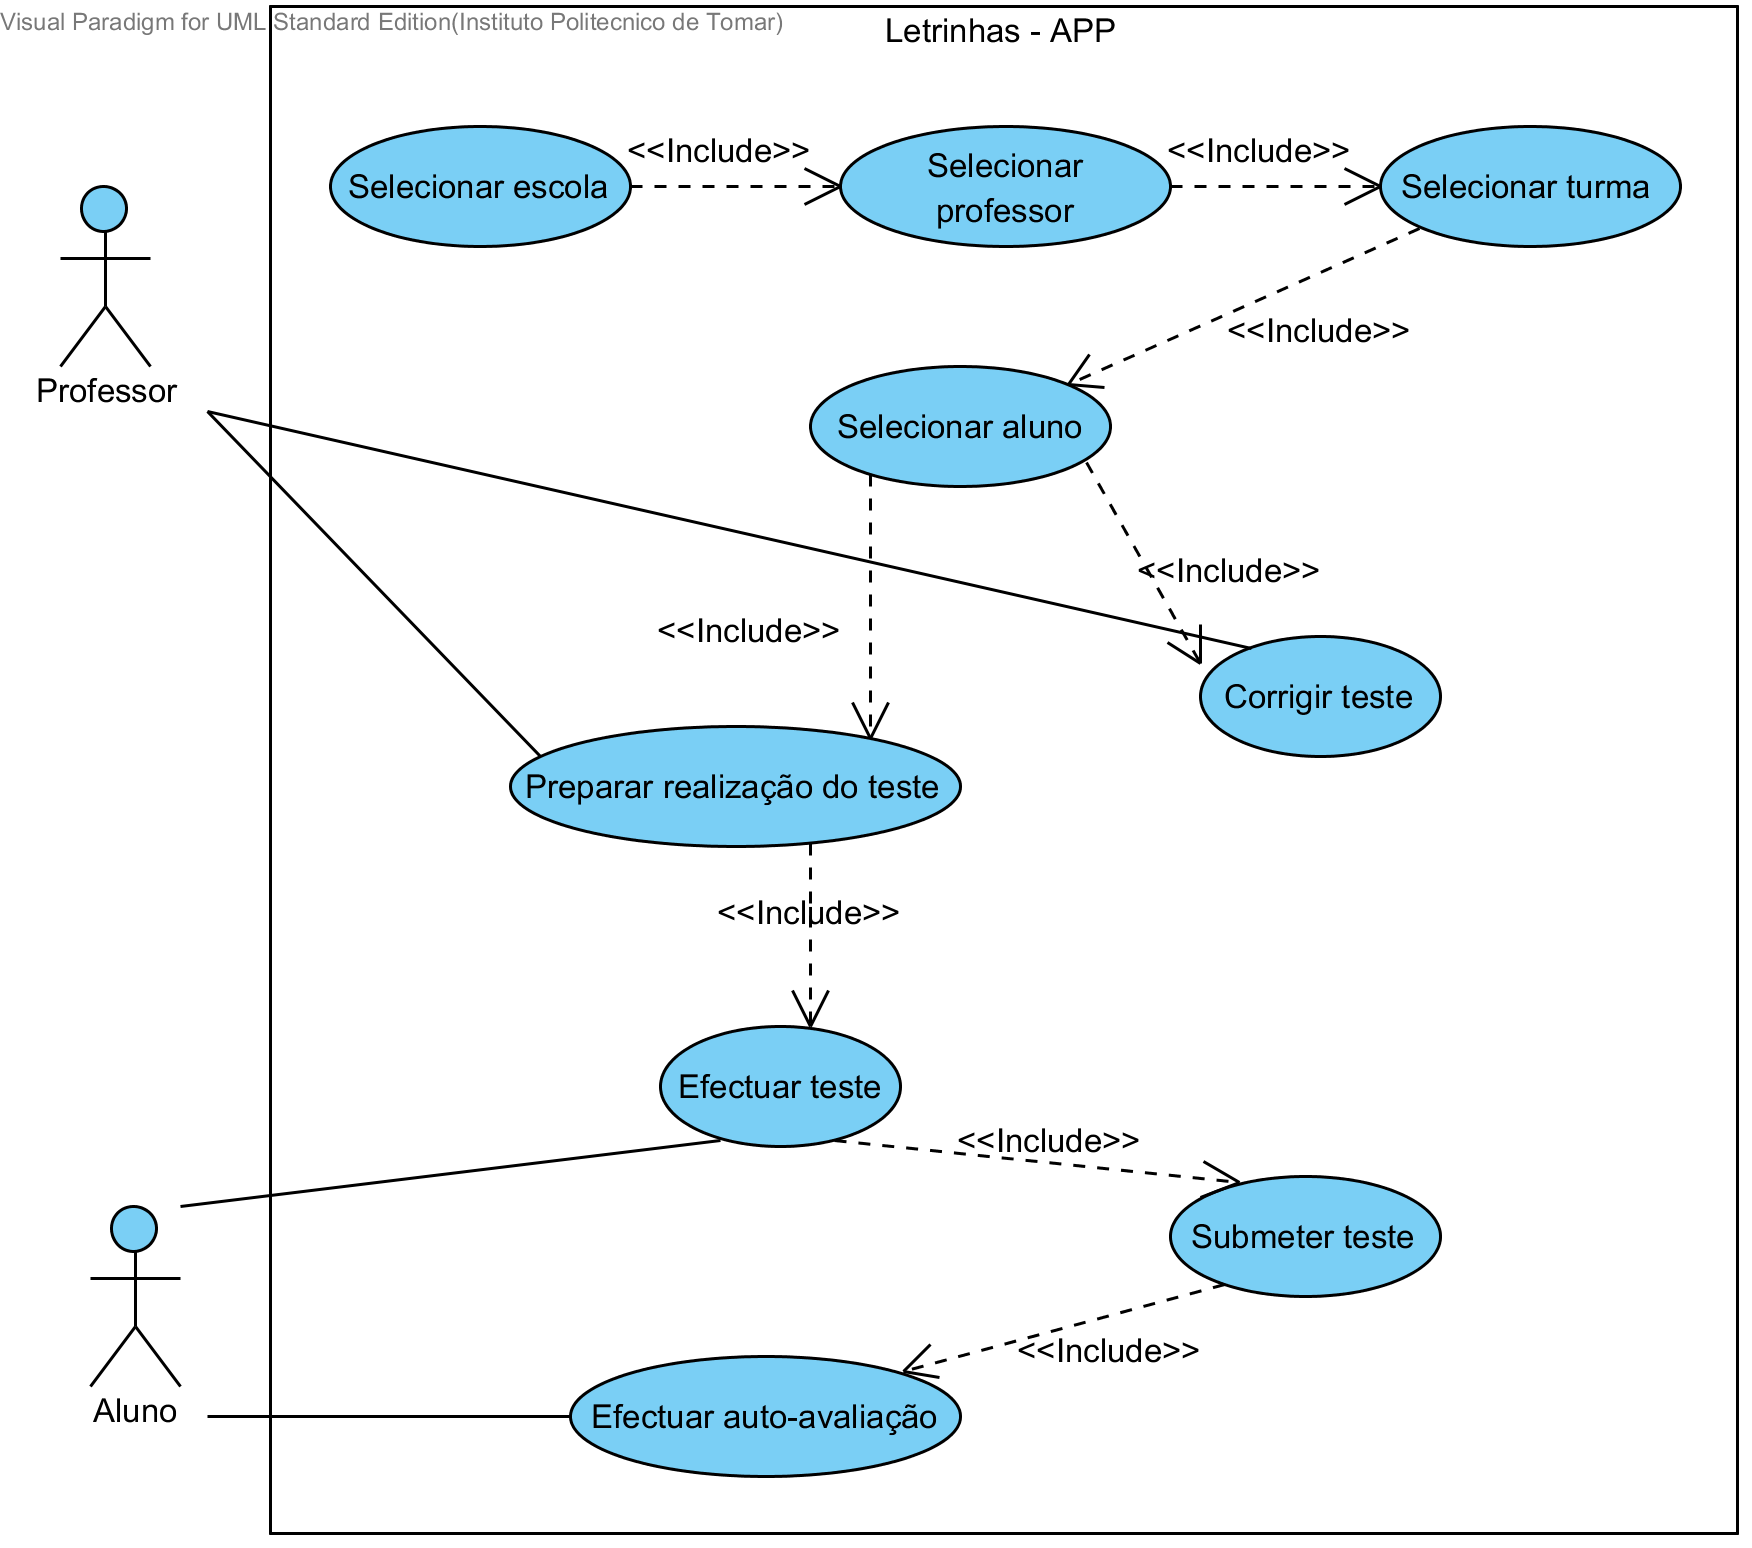
\includegraphics[width=0.8\linewidth]{./diagramasAnaliseSistemas/APP}
				\caption{Casos de Utilização do ator professor e aluno.}
				\label{fig:APP}
			\end{figure}

			Através do diagrama representado na figura 1 podemos observar os casos de utilização do ator professor:
			\begin{itemize}
			\item	Preparar a realização do teste;
			\item   Corrigir teste;
			\end{itemize}
			
			Através do diagrama representado na figura 1 podemos também observar os casos de utilização do ator aluno:
			\begin{itemize}
				\item	Efectuar teste;
				\item   Efectuar Auto-avaliação;
			\end{itemize}
			\newpage
			\subsubsection{Casos de utilização do Sistema de Informação}
						
			\paragraph{Diagrama de CaU do ator administrador e professor}
			
			\begin{figure}[h]
				\centering
				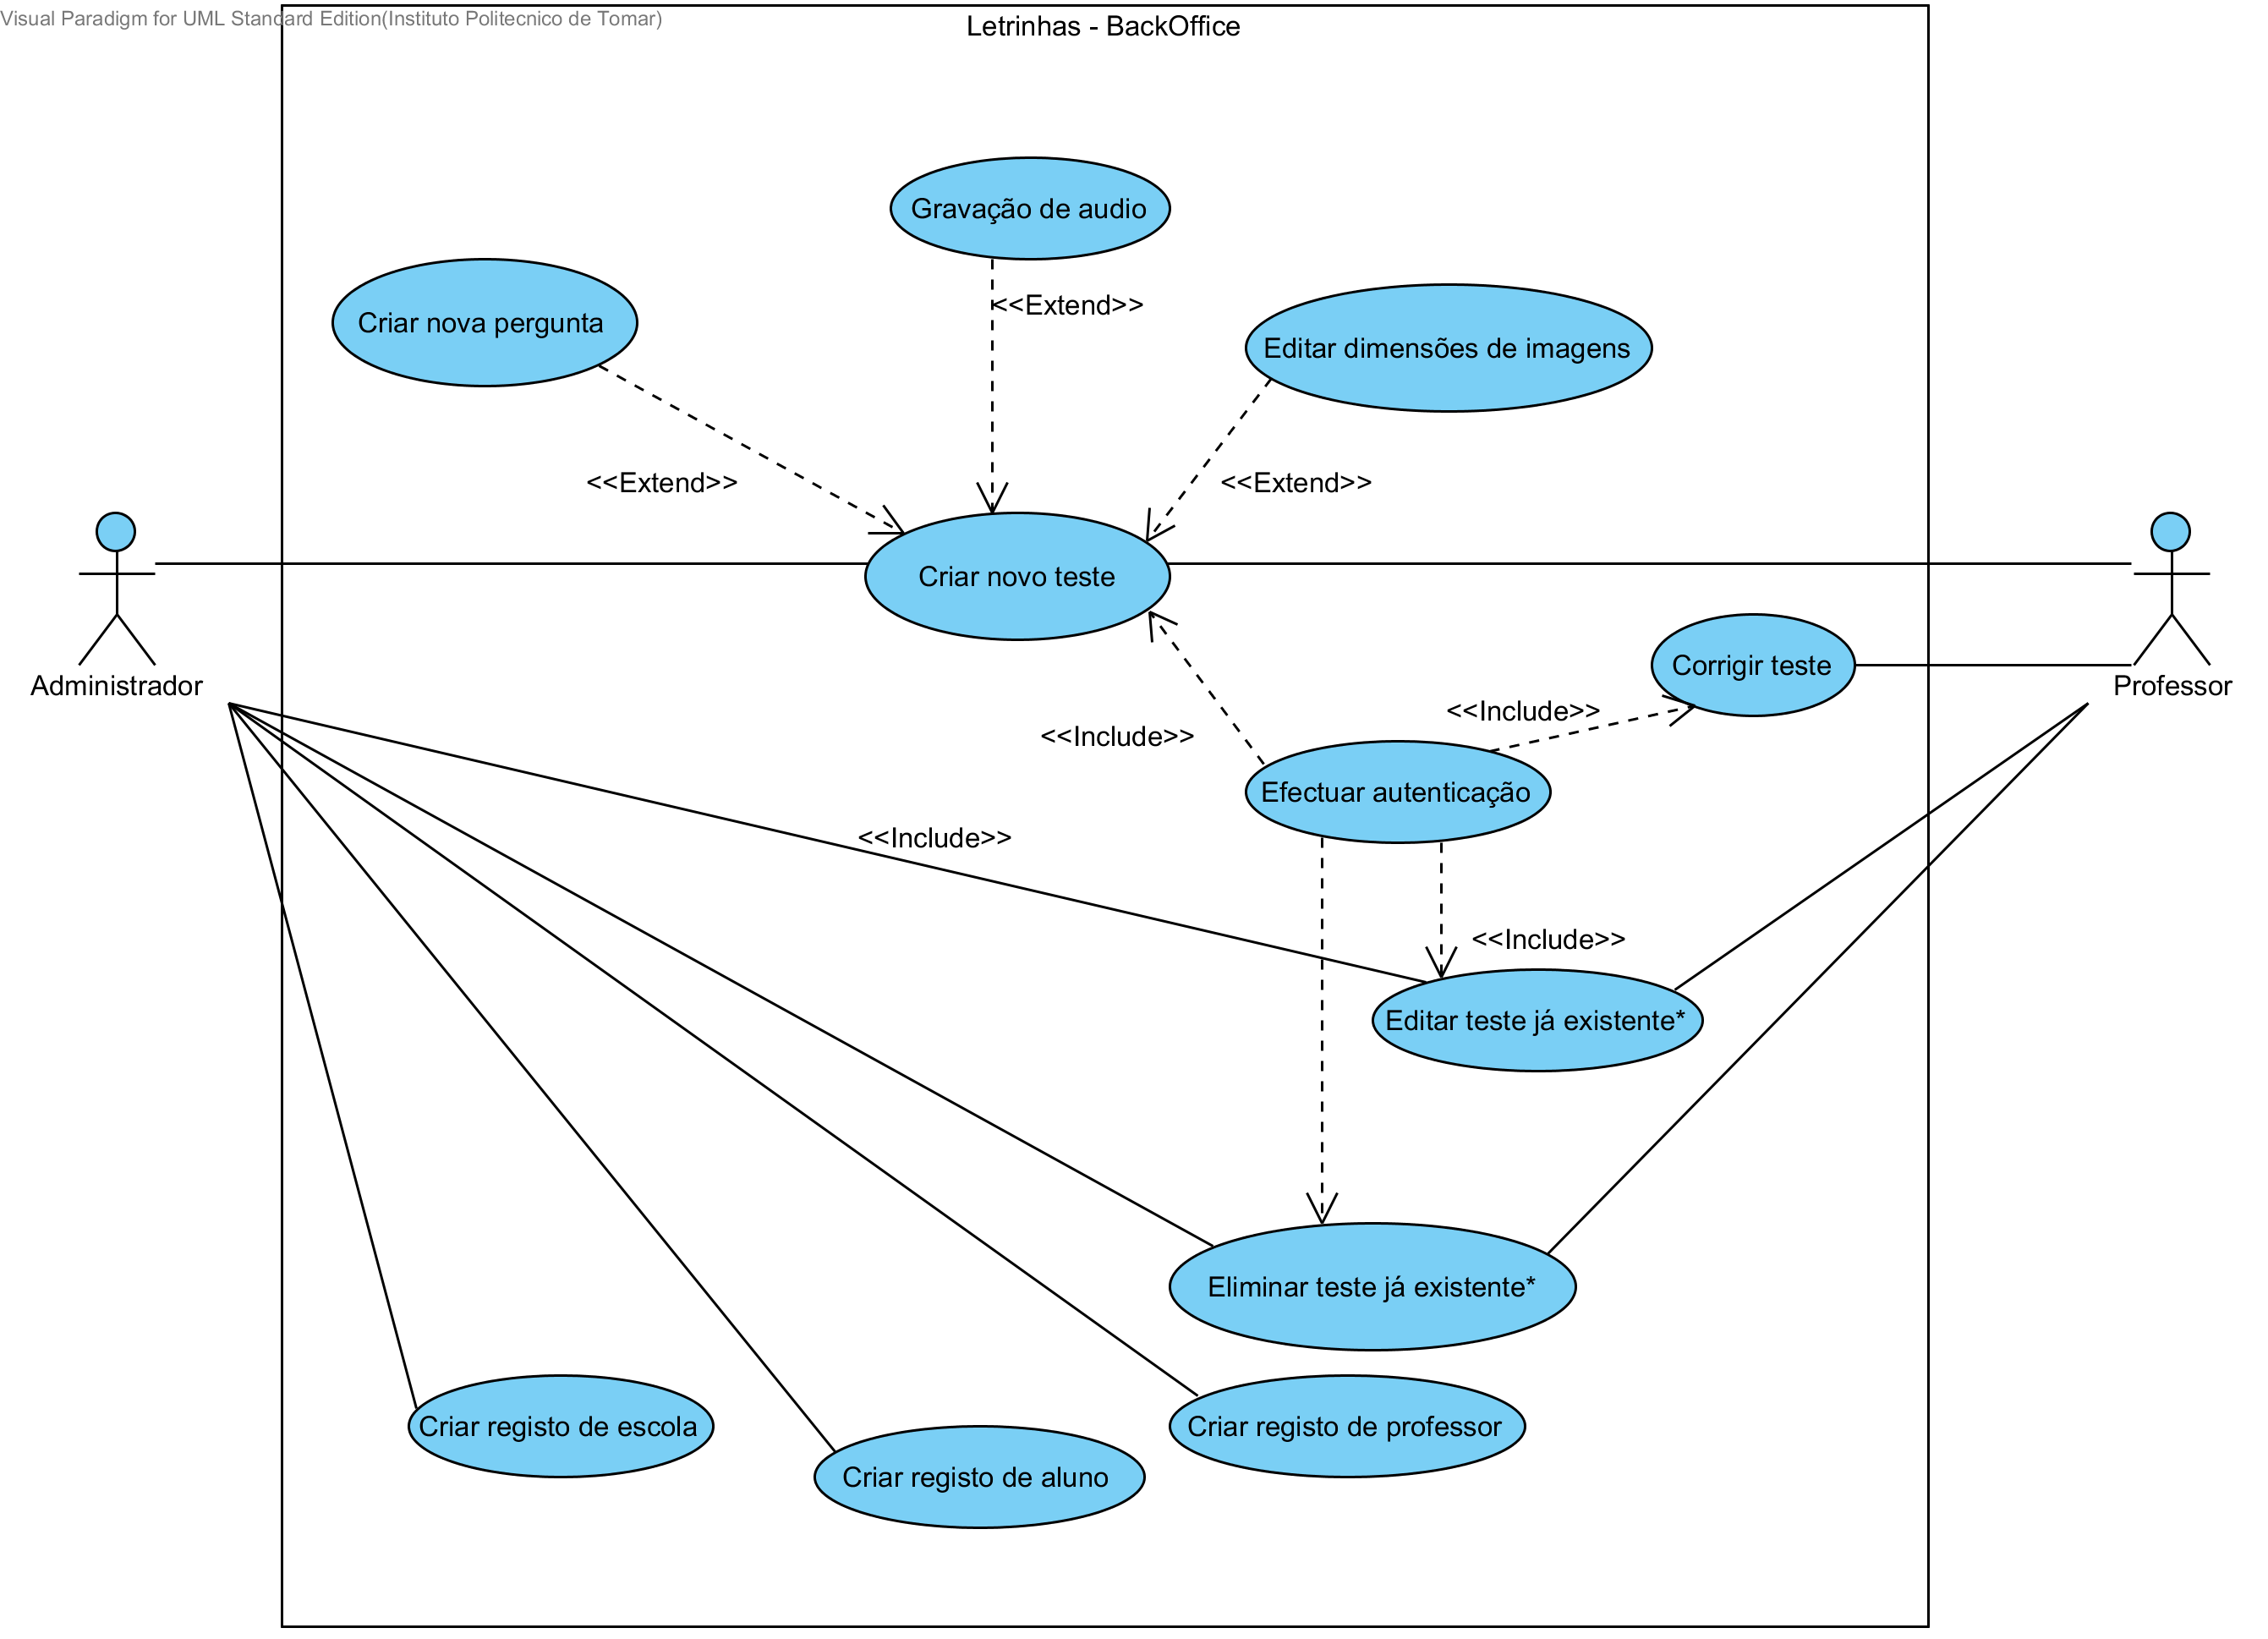
\includegraphics[width=0.8\linewidth]{./diagramasAnaliseSistemas/BackOffice}
				\caption{Casos de Utilização do ator professor e administrador.}
				\label{fig:BackOffice}
			\end{figure}
			Através do diagrama representado na figura 1 podemos observar os casos de utilização do ator adminstrador:
			\begin{itemize}
			\item	Criar novo teste;
			\item   Editar teste já existente;
			\item   Criar registo de professor;
			\item   Criar registo de aluno;
			\item 	Eliminar teste já existente;
			\item   Criar registo de escola;
			\end{itemize}
			
			Através do diagrama representado na figura 1 podemos também observar os casos de utilização do ator professor:
			\begin{itemize}
				\item	Criar novo teste;
				\item   Corrigir teste;
				\item 	Editar teste já existente;
				\item 	Eliminar teste já existente;
				\item   Efectuar Auto-avaliação;
			\end{itemize}
			
			\newpage
			
			\subsection{Descrição dos Casos de Utilização - APP}
					\subsubsection{Corrigir teste}
					\begin{figure}[h]
						\centering
						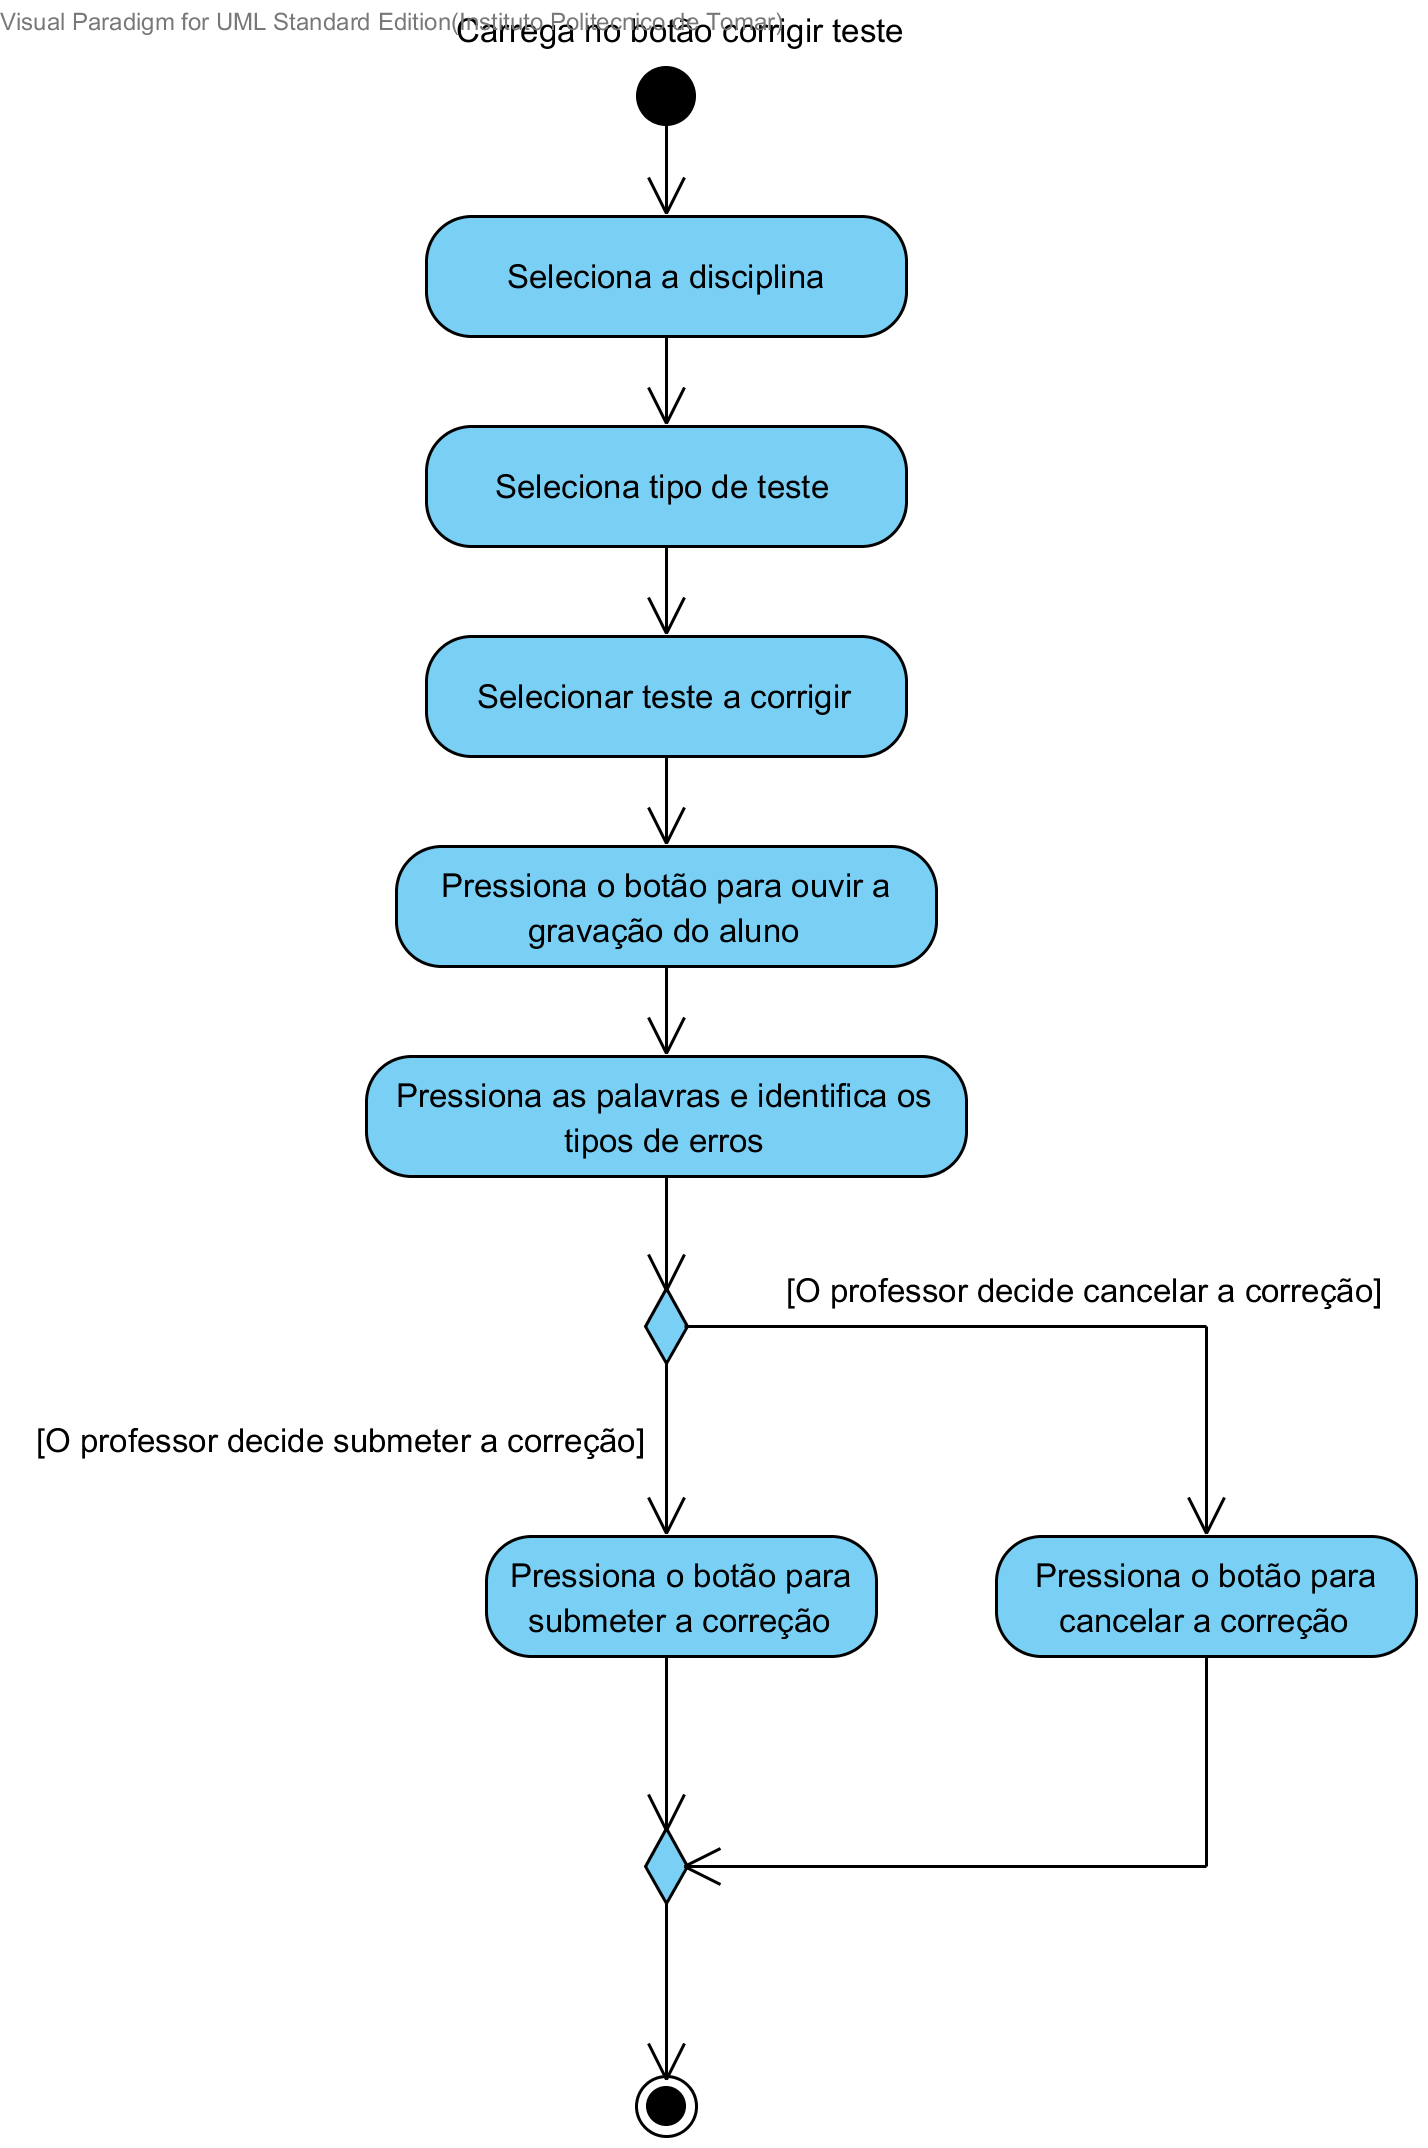
\includegraphics[width=0.7\linewidth]{./diagramasAnaliseSistemas/CorrigirTeste}
						\caption{Diagrama de actividades do C.U. corrigir teste.}
						\label{fig:CorrigirTeste}
					\end{figure}

				\newpage
				\begin {table}[h]
				\begin{tabular}{|p{2cm} p{10cm}|}
					\hline Nome: & CaU Corrigir Teste \\ 
					\hline Âmbito: & Letrinhas - APP \\ 
					\hline Finalidade: & Correcção do teste. \\ 
					\hline Atores: & Professor \\ 
				    \hline Pré-condições: & Deverão existir testes submetidos pelo  aluno.
					O utilizador deverá escolher a  Escola, escolher o professor, escolher a turma, seleccionar o aluno. \\ 
				    \hline Sequência típica dos eventos: &  					
					O utilizador deve:
				    \begin{enumerate}
				    	\item	Seleccionar Corrigir Teste;
						\item	Seleccionar Disciplina;
						\item	Seleccionar o tipo de teste;
						\item	Selecciona o teste a corrigir entre os realizados;
						\item	Ouve a gravação do aluno;
						\item	Corrige;
						\item	Valida a correcção.
				    \end{enumerate} \\ 
  				    \hline Sequências alternativas e extensões: & 
  				    \begin{enumerate}			    	
  				    	\item[4a.] O utilizador cancela a correcção do teste.
  				    \end{enumerate}
  				     \\ 
  				    \hline Requisitos especiais: & Nenhum.\\ 
  				    \hline Aspectos em aberto: & Nenhum. \\
					\hline 
				\end{tabular}
				\caption{Caso de utilização corrigir teste.}
			\end{table} 
			
		\newpage
				\subsubsection{Preparar realização do teste para o aluno}


				
	
	

	
	\newpage
		
		
		
		\section{Modelo do Domínio}
		\subsection{Visão geral}
		
		[mapa de conceitos, i.e., Diagrama de Classes do domínio do problema; classes com atributos  evidentes e associações. Poderá incluir operações. ] 
		
		\subsection{Opções tomadas}
		[Poderá ser necessário acrescentar um texto a descrever o Modelo do Domínio] 

		
		
		
		
		\newpage
		
		\section{Modelo de dados persistente}

			
		
		
		\subsection{Descrição do modelo de dados}
		
		\begin{table}[h]
		\begin{tabular}{|c|c|p{4cm}|p{4cm}|}
			\hline Nome da tabela & Private Keys & Foreign Keys & Referente à tabela \\ 
			\hline User\_table & userId &  &  \\ 
			\hline Post\_table & postId & userId, threadId & User\_table, Thread\_table  \\ 
			\hline Thread\_table & threadId & sectionId & Section\_table \\ 
			\hline Section\_table & sectionId & areaId, sectionParentId & Area\_table, Section\_table \\ 
			\hline Area\_table & areaId &  &  \\ 
			\hline Message\_table & messageId & UserId\_rementente, UserId\_destinatario & User\_table \\ 
			\hline Subsection\_table & sectionId, subsectionId & sectionId, subsectionId & Section\_table \\
			\hline 
		\end{tabular} 
		\caption{Descrição do modelo de dados}
		\end{table}
		
		
		
		
		\newpage

		\section{Protótipo exploratório}
		
		\subsection{Proposta para página inicial do sistema}

		Como referido anteriormente a página inicial deve conter ligações para as seguintes páginas:
			\begin{itemize}
				\item Página de Login;
				\item Página de Registo;
				\item Opção de entrar como guest.
				\subitem Ao escrever "Entrar como convidado" invés de "Entrar como guest", foi uma opção tomada para que se mantenha a consistência desta interface. 
			\end{itemize}
		
\newpage

		
		\section{Plano de Projeto}
		
		\subsection{Escalonamento dos casos de utilização}
		\begin{table}[h]

		
			\begin{tabular}{|c|c|}
				\hline Nome do Use Case & Prioridade \\ 
				\hline &  \\ 
				\hline &  \\ 
				\hline &   \\ 
				\hline &  \\ 
				\hline 
			\end{tabular} 
			\caption{Escalonamento dos casos de utilização }
		\end{table}	
		\newpage	
		\section{Modelo Estrutural}
		
		\subsection{Organização da Solução}
		


		
		\subsection{Tipos de Utilizadores}
		
		Foi tomada a opção de recorrer a um utilizador deste e daquele tipo pois...
		
		\newpage
		
		\section{Anexos}
		
		
					
\end{document}
 